\chapter{总体架构}
本论文的目标是引入深度学习的方法针依据不同工具对代码的检测能力对大量缺陷代码进行分类,在使用多种检测工具对同一份代码进行检测时,可以有效得知这些工具针对这份代码的检测能力,然后利用这些工具的检测报告给出更精准的评判,从而提升检测精度。
\section{设计背景}
随着软件规模的增大,缺陷检测的难度和所需要的代价都越来越大,就Java语言的空指针引用异常的检测来说,目前业界存在着很多工具。如Findbugs,Jlint,Infer,Fortify等。他们在检测缺陷时使用了模式匹配,数据流分析,类型系统,模型检查等技术,由于不同的技术出于对检测精度和效率的权衡,他们所产出的检测报告往往各不相同,并且几乎都包含了大量的误报和漏报,开发人员在面对这样复杂的报告时,很难判断某条报告的准确性。NickRutar[A comparison of Bug Finding Tools for Java]等人针对五种Java语言的缺陷检测工具做了比较,发现没有任何一个单一的工具是完美的,此外,不同工具所产出的报告之间也有不小的差异。

基于这种情况,可以设想将多种工具的报告汇总到一起进行交叉验证,如果多个工具同时给出了同一个位置出现同一种缺陷的报告,我们有理由相信这个缺陷是真实可信的。因此,本文基于sonarqube平台开发了插件BIT-Detector,这个插件集成了Findbugs,Jlint,Infer和Fortify的能力,针对同一份待测代码,首先使用4种工具分别检测并给出报告,然后过滤出空指针引用缺陷,最后将4份报告的内容格式统一化从而进行比对,将不同工具同时检出的空指针引用缺陷作为BIT-Detector的输出,这样的结果理论上可以达到很高的准确率。

由于难以找到合适的空指针引用缺陷数据集,为了对这些工具进行合理的评测,本文采用一种特别的方式构建了一批可信的测试用例,这些用例的构造方法会在后面的章节详细说明。利用构建出来的7429个测试用例,我们针对上文提到的四种工具以及BIT-Detector进行了测试。图\ref{fig:figure3-1}反映了各个工具检出的空指针引用缺陷的重叠情况,表\ref{tab:table3-1}给出了不同工具检测的精度信息,同时还给出了BIT-Detector的数据。通过对比不难发现,各个工具的检测结果确实有较大差异,即使我们使用检测准确度最高的Findbugs,也会面临超过三分之一的误报,这些误报掺杂在检测报告中会给开发人员的缺陷修复带来很多困扰,可能很多时间和精力都会被浪费在验证缺陷的真实性上面。而保证报告的准确性应该是对检测工具的基本要求,即使不谈准确率,过多的漏报也会让人沮丧。显然,目前被广泛使用的各种检测工具还有很大的提升空间。

\begin{figure}
	\centering
	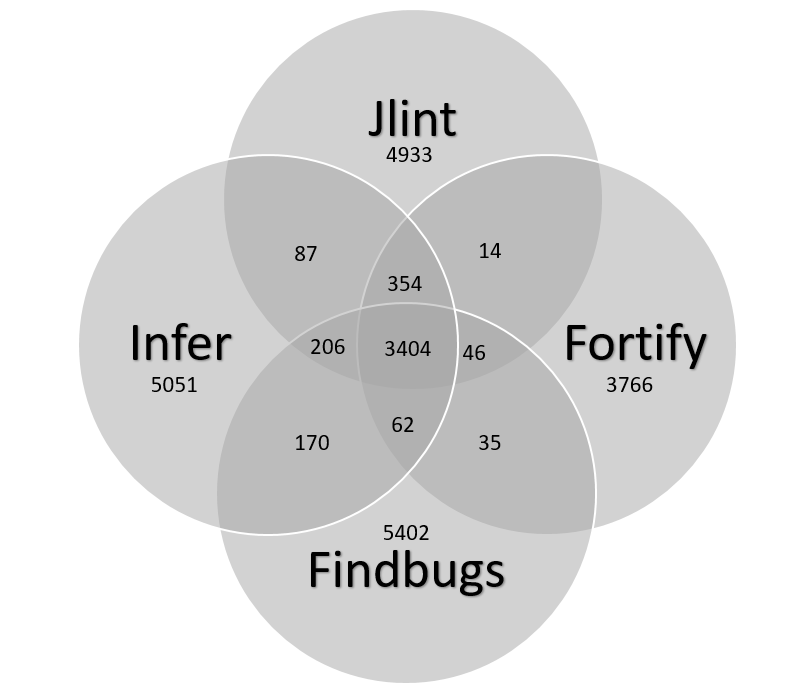
\includegraphics[width=0.70\textwidth]{figures/vnfigure3-1}
	\caption{4种工具在7429个测试用例上的检测结果}\label{fig:figure3-1}
\end{figure}

\begin{table}
	\centering
	\caption{四种工具和BIT-Detector的测试结果对比} \label{tab:table3-1}
	\begin{tabular*}{0.9\textwidth}{@{\extracolsep{\fill}}ccccc}
		\toprule
		测试工具	&正报	&误报	&准确率	&召回率 \\
		\midrule
		Findbugs	&5402	&3169	&63\%	&72\% \\
		Jlint	&4933	&9137	&35\%	&66\% \\
		Infer	&5051	&3578	&58\%	&68\% \\
		Fortify	&3766	&2211	&63\%	&50\% \\
		BIT-Detector	&3404	&576	&85\%	&45\% \\
		\bottomrule
	\end{tabular*}
\end{table}

在检测过程中,我们也注意到选取所有工具共同检测缺陷作为输出结果的BIT-Detector在检测结果的准确率方面有着突出表现,相对于表现最好的Findbugs和Fortify,BIT-Detector有着22\%的准确率提升,而相对于准确率较低的Jlint而言,BIT-Detector的准确率提升则是成倍的增加。即使召回率的表现不尽人意,但是如果我们不将除了四种工具同时检测的缺陷排除在外,而是将四种工具的检测结果按照优先级排序,召回率在某种程度上反而是提升的,如果按照这种方式处理检测报告,此时BIT-Detector的检测结果将自然地排在最前面,但是对其他结果的排序就成了一个棘手的问题,假如我们有四种工具,分别记为$T_a$,$T_b$,$T_c$,$T_d$。如果工具$T$在被测代码的$L$位置成功检出了某个缺陷$D$,则记为$E(T,L,D)=1$,反之则记为$E(T,L,D)=-1$。给定位置$L_i$,存在如下这种情况

\begin{equation*}  
	\left\{  
	\begin{array}{lr}  
	E(T_{a},L_{i},D)=1; &  \\  
	E(T_{b},L_{i},D)=1; &  \\  
	E(T_{c},L_{i},D)=-1; &  \\  
	E(T_{d},L_{i},D)=-1; &  \\  
	\end{array}  
	\right.  
\end{equation} 

在这种情况下,开发人员很难判断位置$L_i$处是否存在缺陷$D$,由上文已知,不同工具对同一份代码的检测结果不同,且它们的检测能力往往不能互相覆盖。所以,对于缺陷$D$,如果我们已知工具$T_a$,$T_b$,$T_c$,$T_d$对该缺陷的检测能力,那么对于检测结果的可信度就可以依据不同工具对于该缺陷的检测能力来确定。如果针对不同的缺陷类型,如空指针引用缺陷,资源泄露缺陷,跨站脚本引用缺陷等对不同工具进行能力评估是比较简单的,只需要计算不同工具在特定类型缺陷上的准确率就能大致评估在该类缺陷上不同工具的检测能力,但是如果只限定在单一的缺陷类型上,例如缺陷$D_1$,$D_2$都是空指针引用类型的缺陷,确定不同工具对缺陷$D_1$,$D_2$的检测能力就是比较棘手的事情了。我们需要找出缺陷$D_1$和$D_2$在代码结构和语义上的不同之处,还需要找出不同工具在检测策略上对这两种缺陷代码处理的不同之处。

显然,利用人工去分类所有空指针引用缺陷是相当困难的事情,分类的种类是否全面,粒度是否精确都会对评估不同工具的能力的结果造成很大影响。面对这种情况,深度学习具备相当不错的解决方案,如前文相关工作中提到的,研究人员已经利用深度学习方法在代码的分类上取得了相当不错的效果,受次启发,本文将利用深度学习的方法评估不同工具对空指针引用缺陷的检测能力。

\section{设计思路}
从上一节设计背景中的讨论可知,不同工具对空指针引用缺陷的检测能力是不同的,而这种能力也并不能很容易地进行评估,这就造成BIT-Detect不能对多个工具的检测报告进行很完美的交叉验证,在检测报告中对于同一位置的缺陷,不同工具可能会给出不同的判定结果,本文提出使用深度学习的方法,在大量缺陷代码数据集的基础上,利用深度神经网络根据代码和工具检测的结果训练出判定不同工具对特定代码检测能力的模型。

深度学习的方法需要大量的训练数据才能得到表现良好的模型,所以首先应该解决开源空指针引用缺陷用例缺乏的问题,然后为了方便后面的数据训练,需要将代码的结构特征转化为数学空间的向量特征,在这个工程中需要解决代码的控制流提取以及代码特征抽取问题,之后可以利用Structure2Vec算法完成图到向量的转化。最后需要给这些数据打标,即通过不同工具的检测得到这些工具在用例上的检测结果,最后将标注过的数据作为模型的输入,完成整个训练过程。

(1)数据集构建

数据集的构建是模型训练所必须的工作基础,在开源项目中很难找到可用的空指针引用缺陷用例。为了达到良好的训练效果,用例应该具备完整的语义,正确的逻辑,多样的代码结构,至少一条可达路径上必然会出现空指针引用缺陷等特点,考虑到后期的处理和训练,作为用例的程序不应过大,恰好包含满足空指针引用缺陷产生的上下文最佳。加上这些要求,在开源环境下直接获得可用的训练数据集就更困难了。

考虑到LeetCode,ACM等具备竞赛性质的项目下可以获得大量代码完整,逻辑正确同时工程精简的代码集,数据集的构建可以通过改造这些代码来完成。为了增加代码的多样性,还可以加入OWASP,ONIST等跟代码缺陷检测相关的项目下的数据集,另外也可以通过人为构造部分数据集作为补充。

(2)控制流图生成

代码的结构化特征可以通过控制流图很好的表达出来,不同程序之间的结构化差异很大程度上可以通过控制流图反映出来,所以生成正确的程序控制流图是后续模型训练的重要保证。

在具备相当数量的缺陷用例数据集后,需要将这些用例的控制流图提取出来。这个过程可以利用现有的工具来完成,例如SOOT,LLVM等工具,它们可以很方便地构造出Java代码的控制流图和方法间调用图,利用这两方面的信息,基本可以提取到代码所有的结构化特征。从本文关注的角度来看,只需要提取出空指针缺陷发生的上下文信息即可,即提取从变量赋值为null到变量被解引用产生异常为止的控制流子图。

(3)代码特征抽取

控制流图只能反映出程序的结构化信息,对于空指针引用缺陷的检测来说,工具需要更多地理解代码的语义信息,一个赋值语句的差别可以很容易地决定是否能够产生空指针引用缺陷。如果要体现程序的语义信息,需要尽可能多地抽取出每一句代码的静态特征,如是否将null赋值给了变量,是否针对null值进行了检查,是否调用了其他方法等。这些特征将附着在控制流图的每一个结点上,为后续的模型训练提供更多的代码特征信息。这些工作同样可以利用SOOT,LLVM等工具来完成。

(4)数据标注

对于一个给定的程序片段,模型理想的输出结果为不同工具分别是否具备检测该段代码的能力,即这些工具检测结果的可信度。那么本方案中数据的标签即是不同工具对该用例实际检测的能力,即是否能够检测出该用例设计的缺陷。这个标注过程可以利用上节提到的BIT-Detector插件来批量完成。

(5)模型训练

模型训练大致可以分为两部分,第一部分利用Structure2Vec算法对上述步骤中产生的包含特征向量信息的代码控制流图向量化,第二部分将这些向量化后的图向量和相应的标签一起针对不同的工具分别进行分类训练。每个模型都可以针对给定的代码判断该工具能否正确检测出缺陷。

(6)结果验证

最后,可以利用不同工具的模型得到它们对于待测代码能否检测出缺陷的能力判断,综合这些工具在该代码上实际的检测结果,可以得到该代码是否具备缺陷的最终判定。

\section{整体架构}

本文的最终目的是基于sonarqube平台开发一种空指针缺陷引用检测系统,下面简单介绍一下该系统的运行模式,如图\ref{fig:figure3-2}所示,SonarQube平台可以非常方便地与开发人员使用的IDE,代码版本管理工具以及持续集成框架集成在一起。将这些工具整合到一起之后的工作流大致有如下步骤:

\begin{figure}
	\centering
	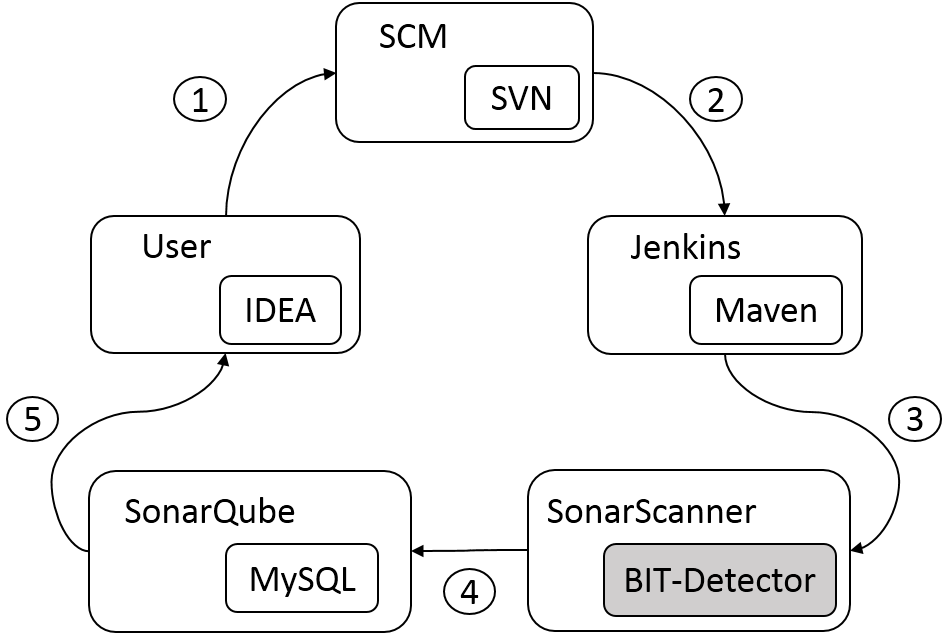
\includegraphics[width=0.70\textwidth]{figures/sonarqube3-2}
	\caption{SonarQube平台工作流程}\label{fig:figure3-2}
\end{figure}


(1)用户在IDE中完成代码编辑之后推送代码至SCM(SoftWare Configuration Mangement)仓库,选用的工具可以是SVN,Git等。

(2)Jenkins通过配置可以与核心仓库中的代码进行同步,并能感知仓库代码是否生了变动。

(3)Jenkins在感知到核心仓库的代码发生改变之后,自动触发代码构建动作,构建工具可以选用Maven,Gradle等。代码成功构建之后,Jenkins会触发SonarScanner扫描代码的操作。

(4)SonarScanner首先加载配置文件记录的代码位置及目录结构信息,然后由插件负责对代码进行全面检测,并生成检测报告。最后检测报告将按照特定格式传递给SonarQube服务器。

(5)SonarQube服务器会处理SonarScanner传递的代码检测报告,并将报告数据存储在MySQL等数据库中,一个工程同时可以拥有多份不同批次的检测报告,最后这些报告将会以合适的方式可视化给用户查阅。

本文重点介绍BIT-Detector的部分设计开发工作,BIT-Detector是以插件的形式在SonarScanner中承担着检查代码的工作。它的主要工作流程如图\ref{fig:figure3-3}所示。首先,用户需要针对特定的工程配置好sonar-scanner.properties文件,文件中记录了工程的名称,SonarQube项目的代号,版本等基本信息,还有工程的源码,测试代码及编译后的字节码文件所在目录和依赖库等信息的位置。这些信息将提供给插件中的代码检测工具使用。在获得必要的信息之后,调用不同的工具对代码进行检测,然后根据不同工具的特性收集相应的检测报告。不同的工具所产生的报告格式也是不一样的,在交叉验证阶段,需要将这些报告的格式统一处理,同时还需要过滤掉不需要的缺陷类型,例如本文重点关注空指针引用缺陷,只需要留下空指针引用缺陷类型即可。后面就可以根据汇总的缺陷数据对检测报告进行粗略的分类,将所有工具都能检测出来的缺陷选取出来,作为最高优先级的缺陷,其他缺陷需要经过模型进行进一步的验证。需要模型验证的用例需要确定分析域范围,即空指针产生的上下文,这些信息可以通过代码检测工具得到,然后提取出这部分的控制流图,抽取出代码特征,在通过模型进行向量化之后可以利用训练好的分类器得到不同工具对该代码的检测能力评价,即工具的置信度。利用工具的置信度可以对工具检测的结果进行适当修正,并根据可信程度对缺陷进行进一步的排序。最后将报告提交给SonarQube进行可视化输出。

利用模型评价工具的检测能力是本文重点研究的部分,后续的章节将会重点介绍模型训练相关的工作,其他关于插件开发的工作不再过多阐述。


\begin{figure}
	\centering
	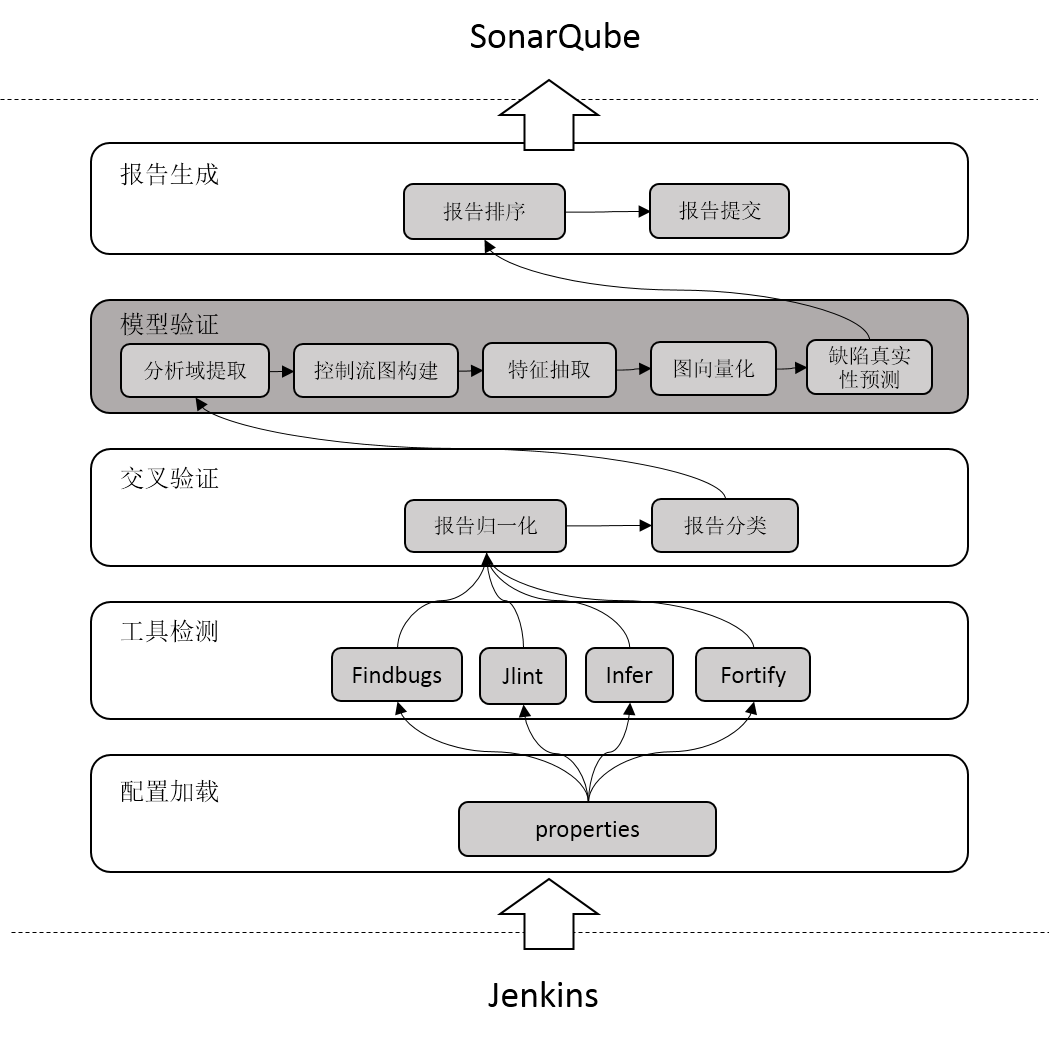
\includegraphics[width=0.80\textwidth]{figures/BITDetector3-3}
	\caption{BIT-Detector工作架构图}\label{fig:figure3-3}
\end{figure}

\section{本章小结}

本章介绍了BIT-Detector的设计背景,详细讨论了该工具的设计思路,特别交代了在工具中引入深度学习方法的原因。之后介绍了基于SonarQube平台的代码检测流程,重点介绍了BIT-Detector的架构设计和工作过程,最后阐明全文研究的重点聚焦在深度学习模型的实现和训练上面。
